\documentclass[10pt]{article}
\usepackage{typoday18}

\title{Spiral splines in typeface design - A case study of Manjari Malayalam typeface}

\author{ 
 Santhosh Thottingal
  \and
 Kavya Manohar
}
 

\begin{document}

\maketitle

\begin{abstract}

Manjari typeface was an experiment to use spiral splines to define the curves of Malayalam glyphs. It was a milestone in the progression of script towards maximally rounded glyphs. The script has been evolving from its rectangular characteristics in the early days of metallic types to the circular characteristics of popular digital fonts. 

The design of curves in Manjari are theoretically based on the PhD thesis by Raph Levien - “From Spiral to Spline: Optimal Techniques in Interactive Curve Design”\footnote{\url{http://www.levien.com/phd/}}. The design process relied almost entirely on the spiro toolbox developed  by Levian himself, available as free software library in Inkscape vector graphics editor.

The use of spiral spline curves resulted in shapes that are extra smooth. The spiral smoothness of curves are complemented by rounded terminals which gives very soft feeling for the eyes. The rigidness of geometric fonts is completely avoided and  the Manjari font has a good humanist identity. The curve perfection resulted in negative spaces that aquired beautiful leaf and drop shapes between the bowls and loops of the script. 

In this paper we present the design principles and aesthetic concepts behind this font along with a perspective on the evolution of script aesthetics from the ancient writing systems, through early and contemporary printing to digital fonts. We will also see the popularity and adoption of Manjari in the digital as well as print media.
\end{abstract}
 \textbf{Keywords:} Malayalam, Script, Spirals, Opentype, Typeface, Digital Typography

\section{Introduction}

Malayalam script, since its journey from Brahmi\footnote{\url{https://www.britannica.com/topic/Brahmi}} writing style through Vattezhuthu and Grantha\footnote{\url{https://www.britannica.com/topic/Grantha-alphabet}} writing systems to the digital typefaces of modern era, has undergone a lot of changes. The noticeable aesthetic feature of contemporary script is its loops and curly strokes. Horizontal symmetry for many letters like {\rachana {ക, ത, ന}} became an identity for the script. Manjari Malayalam typeface utilises spiral shapes to accentuate these features that resulted in its aesthetic acceptance. A sample of text rendered in Manjari typeface is shown in Figure. \ref{wordcloud}. 

\begin{figure}[h!]
	\centering
	\includegraphics[width=\textwidth]{images/wordcloud.jpg}
	\caption{Text rendered in Manjari typeface}
	\label{wordcloud}
\end{figure} 

\section{Evolutionary Path of the script}

Samples of copper plate inscriptions and palm leaf manuscripts show that the letters were never perfect rounds, but rather rectangular or elongated curves. The sample shown in Figure.\ref{vattezhuthu} is inscription from Tharisappalli copper plates dating back to 849 AD.


\begin{figure}[h!]
	\centering
	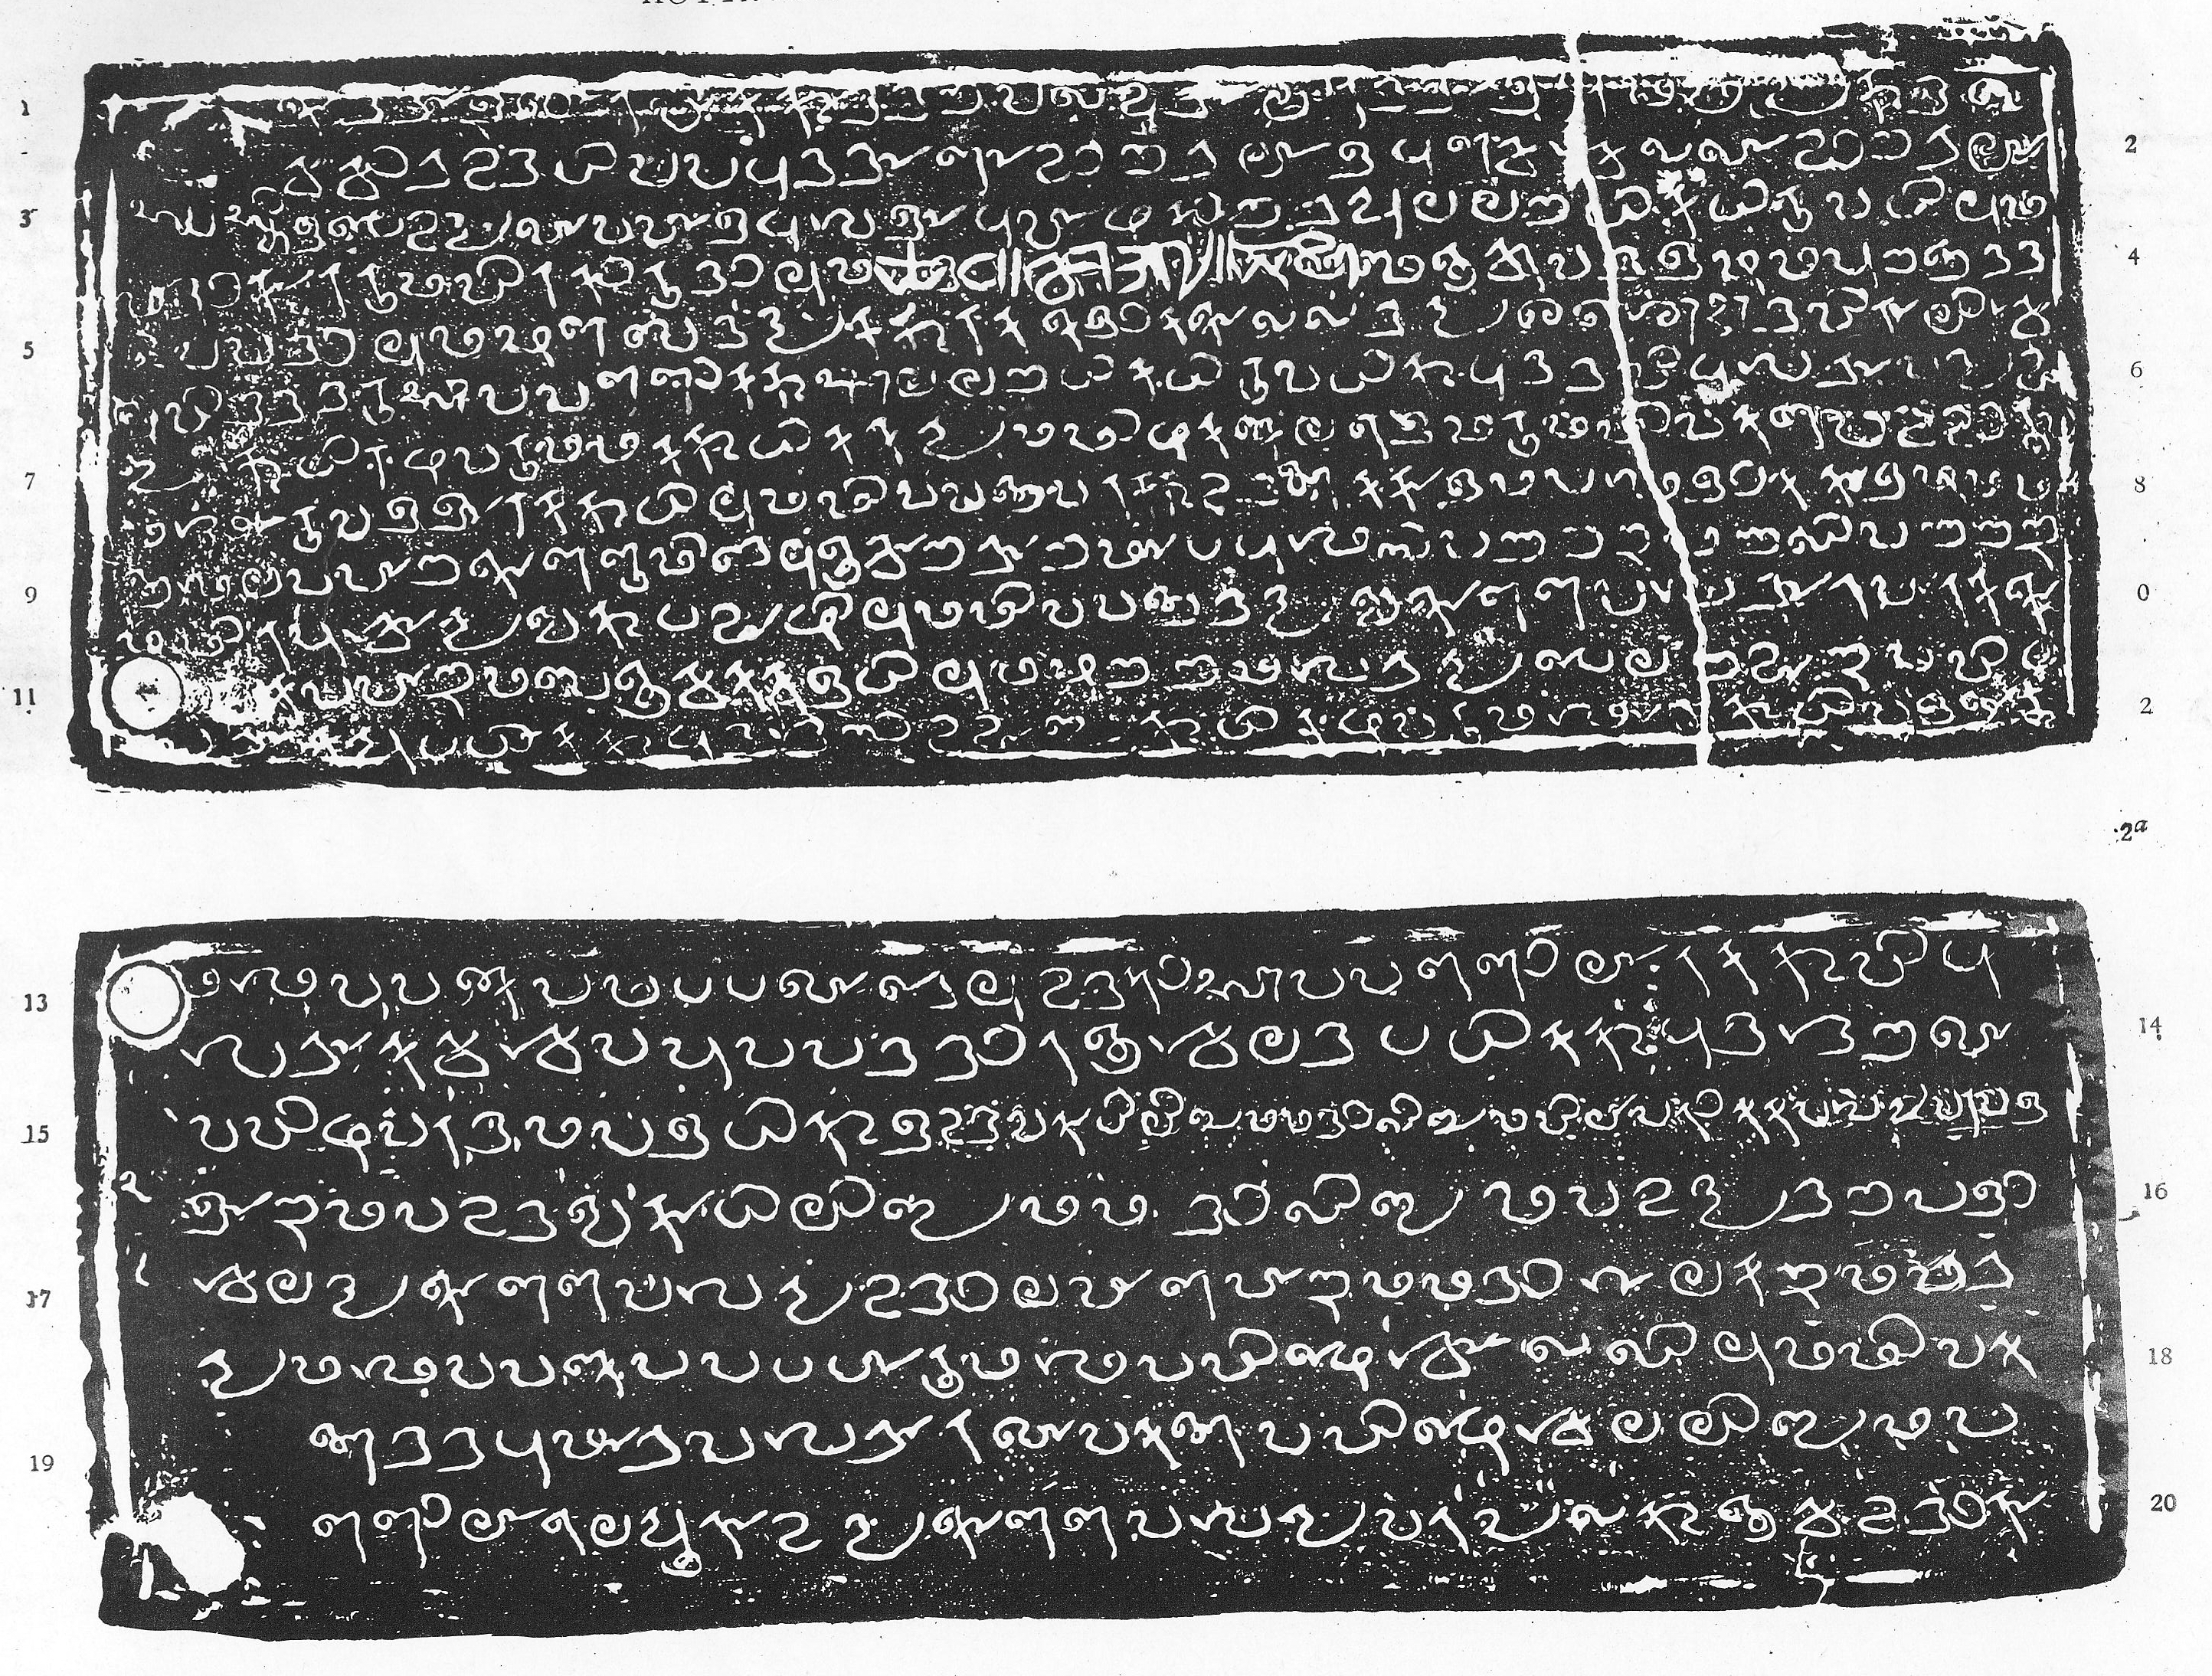
\includegraphics[width=0.6\textwidth]{images/Tharisappalli_copper_plates.jpg}
	\caption{Copper plate inscription in Vattezhuthu.}
	\label{vattezhuthu}
\end{figure} 


The rectangular nature of the script was its characteristic during the early days of printing. The first ever printed Malayalam book was Samkshepavedartham, printed in Rome using movable types in 1772. Sample pages of the book is shown in \ref{Samkshepam}. 



\begin{figure}[h!]
	\centering
	\includegraphics[width=0.8\textwidth]{images/samkshepavedartham1772.png}
	\caption{Samkshepavedartham-1772 shows rectangualar nature of glyphs in early print}
	\label{Samkshepam}
\end{figure} 

Next remarkable event in history of Malayalam typefaces occured when movable types were casted natively in Kerala, India during 1829 by an Anglican Missionary Benjamin Bailey\cite{babucherian} for CMS Press, Kottayam, Kerala. These metal types were close to perfect round and the popularity of books from this press started to give uniform height proportions to the script. According to Gupthan Nair, Bailey's contributions as a typographer made the curvy style of the Malyalam script popular\cite{gupthannair}. See the most impactful output from the CMSpress Kottayam in Figure.\ref{newtestament}, a translation of the Bible.


\begin{figure}
	\centering
	\includegraphics[width=0.8\textwidth]{images/newtestament1829.png}
	\caption{New Testament - 1829}
	\label{newtestament}
\end{figure}

The accepatance of this style of roundness can be easily understood when a fine handwriting is often referred as {\manjari {അവൾക്കു നല്ല ഉരുണ്ട കയ്യക്ഷരമുണ്ട്} } (She has a fine round shaped handwriting).


\subsection{Digital typefaces}

ASCII based non-standard samples. (Added based on some discussion in {\manjari കമ്പിയില്ലാക്കമ്പി} on the infographics made) 

Unicode fonts for regular use: Meera, Anjali - early popular ones.  Their rounded characteristic curves, but sharp edges

Manjari- 2016. Curvature has maximally spiral features. rounded terminals.  Ever since the typeface was released in July 2016, it became one of the top used unicode typeface for Malayalam. Manjari is available in 3 style variants and available publicly under free software license. 

\section{Curve Interpolation by Spiral splines - 25 \% of content}

Curve interpolation.

Different types of interpolation- Mathematical characterisics

Special features of spiral spline- Sample Images

Ralph Levian studies and results. 

The Inconsolata monospace humanist latin font known for its clean lines and elegant design by Levien himself is based on this theory.

\paragraph{Fonts variants by interpolation}
Many interpolating splines in the literature are used for generating variations in fonts, rather
than a single static shape. Since fonts are desired in a wide range of weights, one of the more
common applications is to generate these continuously. One of the most straightforward techniques,
pioneered by Ikarus [42], is to start with two masters with similar structure, representing thin
and thick extremes, and linearly interpolate the positions of the control points between the two.
Then, an interpolating spline is fit through these control points. Note that there are two senses of
interpolation here – one for the control points, another for the spline." \cite{lamport94}


\section{Manjari and its Spiral features - 35 \% of content}

Curves Defined by spiral interpolation

Round edges: Smooth feeling

Equal widtn stroke

\subsection{Beutiful features in the negative spaces}

Sample images.

\includegraphics[width=\textwidth]{images/Manjari-Specimen.pdf}

\section{Free software tools- 10 \%}

Spiro library by Ralph Levian.

Incorporation in inkscape

Version controlled, open source work flow.

\section{Conclusion- 10 \%}

\begin{thebibliography}{99}
	\bibitem{babucherian} Babu Cheriyan, \textit{Benjamin Bailiyum Malayala Sahithyavum} {\manjari{(ബെഞ്ചമിൻ ബെയിലിയും മലയാള സാഹിത്യവും}) }, Mahatma Gandhi University, Kottayam, 2008
	\bibitem{gupthannair} S. Gupthan Nair, \textit{Gadyam Pinnitta Vazhikal}{\manjari{ (ഗദ്യം പിന്നിട്ട വഴികൾ)} }, DC Books, Kottayam 

	
\end{thebibliography}


\end{document}
